\documentclass[journal=jctcce,manuscript=article, layout=twocolumn]{achemso}
\usepackage[table]{xcolor}
\usepackage{amsmath}
\DeclareMathOperator*{\argmin}{arg\,min}
\usepackage{graphicx}
\usepackage{float}
\graphicspath{ {./FIGs/} }

\author{Niccol\`{o} Ricardi}
\email{Niccolo.Ricardi@unige.ch}
\author{Cristina E. Gonz\'{a}lez-Espinoza}
\email{Cristina.GonzalezEspinoza@unige.ch}
\author{Tomasz Adam Weso\l{}owski}
\email{Tomasz.Wesolowski@unige.ch}
\affiliation[University of Geneva]
{Department of Physical Chemistry, University of Geneva, Geneva (Switzerland)}

\title[Negativity of the target density]
  {Negativity of the target density in practical Frozen-Density Embedding Theory based calculations}

\newcommand{\nr}[1]{\color{red}#1\color{black}}    
\begin{document}

\begin{tocentry}

TOC to be made. Probably isosurfaces of target density.

\end{tocentry}


\begin{abstract}
Tentative abstract
\end{abstract}

%%%%%%%%%%%%%%%%%%%%%%%%%%%%%%%%%%%%%%%%%%%%%%%%%%%%%%%%%%%%%%%%%%%%%
%% Start the main part of the manuscript here.
%%%%%%%%%%%%%%%%%%%%%%%%%%%%%%%%%%%%%%%%%%%%%%%%%%%%%%%%%%%%%%%%%%%%%
\section{Introduction}
Frozen-Density Embedding Theory (FDET)\cite{Wesolowski2008, Wesolowski1993} is a multiscale method where the environment is described solely by means of its electron density $\rho_B(\mathbf{r})$ while a wavefunction $\Psi_A$ models the system of interest.
The FDET energy ${E}_{v_A,v_B}^{FDET}[\Psi_{A},\rho_B]$ is defined as:
\begin{align} \label{eq:E_FDET}
{E}_{v_A,v_B}^{FDET}[\Psi_{A},\rho_B] = & \langle\Psi_{A}\vert \hat{H}_A\vert \Psi_{A}\rangle + E^{HK}_{v_B}[\rho_B] + \\ \nonumber
& E^{elst}_{int}[\rho_A,\rho_B] + \\ \nonumber
& \Delta F[\rho_A] + E_{xcT}^{nad}[\rho_A,\rho_B]. 
\end{align}
The first two terms are energy contributions from the two subsystems, represented by the expectation value of the isolated Hamiltonian for subsystem A, and the Hohenberg-Kohn energy of subsystem B.
$E^{elst}_{int}[\rho_A,\rho_B]$ is the sum of electrostatic interactions between the two subsystems:
\begin{align} \label{eq:E_elst_int}
E^{elst,int}_{v_A,v_B}[\rho_A,\rho_B] & = V_{N_{A},N_{B}} + \int {\rho_A(\vec{r})v_B(\vec{r})}d\mathbf{r} + \\ \nonumber
& \int {\rho_B(\vec{r})v_A(\vec{r})}d\mathbf{r}   + \\ \nonumber
& \int\int \frac{\rho_A(\vec{r})\rho_B(\mathbf{r}')} {\left\vert \mathbf{r}-\mathbf{r}'\right\vert}d\mathbf{r}'d\mathbf{r}.
\end{align}
where $\rho_A(\mathbf{r})$ is the electron density associated to the wavefunction, according to $\rho_A(\mathbf{r}) = \vert \Psi_A \vert^2$
The last two terms guarantee a quantum treatment of the whole supersytem. $\Delta F[\rho_A]$ is a term\cite{Aquilante2011} related to the form of the wavefunction $\Psi_A$, which for Hartree-Fock is equal to the correlation $E_c$.
Finally, $E_{xcT}^{nad}[\rho_A,\rho_B]$  is obtained as:
\begin{align} \label{eq:E_xct_nad}
 E_{xcT}^{nad}[\rho_A,\rho_B] = & E_{xcT}^{}[\rho_A+\rho_B] - E_{xcT}^{}[\rho_B] - \\ \nonumber
 & E_{xcT}^{}[\rho_A],
\end{align}
where $E_{xcT}[\rho] = E_{xc}[\rho] + T_s[\rho]$.

By virtue of the second Hohenberg-Kohn theorem:
\begin{equation}\label{eq:fund}
 E_{v_A,v_B}^{FDET}[\Psi_{A}^{o},\rho_B] =  E_{v_{AB}}^{HK}[\rho_A^{o}+\rho_B] \ge E_o,
\end{equation}
where
\begin{equation} \label{eq:Psi_o}
 \Psi_{A}^{o} = \argmin E_{v_A,v_B}^{FDET}[\Psi_{A},\rho_B].
\end{equation}
If we define a target density $\rho^t(\mathbf{r}) = \rho_o(\mathbf{r}) - \rho_B(\mathbf{r})$, it is apparent that the second part of Eq.~\ref{eq:fund} becomes an equality if and only if $\rho_A^{o}(\mathbf{r}) = \rho^t(\mathbf{r})$. This, in turn, is only possible if $\forall \mathbf{r} \ \rho^t(\mathbf{r}) > 0$. 

Such condition, which we will name non-negativity of the target density, cannot be enforced in practical calculations, where $\rho^o(\mathbf{r})$ is not available. Hence, $E_{v_A,v_B}^{FDET}[\Psi_{A}^{o},\rho_B] > E_o$. There have been examples in the literature where FDET was applied with a non-negative target density\cite{Wesolowski2013} or with one where the negativity was minor and only due to numerical effects\cite{Fux2010}. There have not been, although, analyses on the effect of the negativity of target densities in practical calculations.

The aim of this manuscript is hence to assess if there is a relation between some measurement of the extent of the violation of the non-negativity of the target density condition and ${E}_{v_A,v_B}^{FDET}[\Psi_{A},\rho_B]$.

In FDET, the total system is modeled by means of the two subsystem density, but the division is arbitrary. Furthermore, neither density needs to be spatially constrained, and consequently there is no need for a division of the total space into subsystem spaces. Charge transfer and polarization, on the other hand, rely on such a division. Consequently, these concepts are not defined in FDET. Nonetheless, they are clearly linked to the non-negativity of the target density condition.
Let us consider the case of a charge transfer complex where, upon complexation, electron density moves from subsystem B to subsystem A. Any $\rho_B(\mathbf{r})$ localized around what would be the spatial region of subsystem B would violate lead to a negative target density. The same reasoning applies to a charge transfer from B to A upon excitation.
Charge transfers from A to B, be it upon complexation or upon excitation, do not pose a problem in FDET: since the division into A and B is arbitrary, $\rho_A$ can increase in the spatial region of subsystem B.
Similar considerations can be applied on polarization: let us consider the case where $\rho_B(\mathbf{r})$ is the isolated density of subsystem B. Upon complexation the subsystem will polarize, i.e. its density will rearrange. The regions where the environment density decreases will cause our chosen will cause our chosen $\rho_B(\mathbf{r})$ to be larger than $\rho_o(\mathbf{r})$, leading to a negative target density. Analogously to charge transfer, the same considerations apply to the polarization of the density upon excitation.

Due to these considerations, this manuscripts also investigates the relation between different treatment of polarization and the negativity of the target density.

To this end, we analyzed the 4 systems from Ref.~\citenum{Ricardi2018}, which in turn were selected from the 52 structures of Ref.~\citenum{Zech2018}. These systems display different strength of interaction, number of molecules in the environment, number of non-covalent interactions, charge of the environment, etc...
Specifically, 7-hydroxyquinoline bound to 2 methanol molecules (7Hq 2MeOH) and uracil bound to 5 water molecules (Uracil 5H$_2$O) can be considered examples of ``standard'' interactions, as the groups involved in the hydrogen bonding are neutral hydrogen donors and acceptors. In the cases of 7-hydroxyquinoline bound to formate (7Hq formate) and pyridinumyl benzimidazolide bound to 2 formic acid molecules (PyrBnz 2HCOOH) represent more peculiar cases. In the former case, the environment acts as the hydrogen acceptor and is negatively charged. Additionally, the hydrogen bond distance (1.36 \AA) is comparable to that of its covalent bond (1.09 \AA). We have discussed in Ref.~\citenum{Zech2018} how this poses a challenge due to the large overlap of the subsystem densities. In the case of PyrBnz 2HCOOH subsystem A acts as hydrogen acceptor and the atom involved carries a significant negative charge.
In our previous work and in this manuscript, in both full and abbreviated naming, the system of interest always precedes the environment.

\subsection{Measurement of the violation}
In order to investigate the relation between negativity and energy, a parameter needs being chosen which accounts for the extent of the violation of the non-negativity of the target density condition.
To this end, we decided to integrate the target density only where it is negative, according to:
\begin{equation}\label{eq:M}
  M[\rho_{t}] = -\int \rho^{t}(\vec{r})\cdot \Theta(-\rho^{t}(\vec{r})) \ d\vec{r},
  \end{equation}
where $\Theta$ is the Heaviside step function. The resulting values are bound between 0 and $\int \rho_B = N_B$. \nr{Maybe elaborate on why?}
\section{Approximate FDET-based methods}
The discussion has so far focused on theory. In such case the only factor inducing an error $\Delta E = E_{v_A,v_B}^{FDET}[\Psi_{A}^{o},\rho_B] - E_o$ is the negativity of the target density. 
In most practical calculations though, neither of these two quantities is available.

Some approximation has to be chosen to obtain $E^{ref} \approx E_o$. Generally, the same approximation is used for $\hat{H}_A$ in the embedding procedure.
Furthermore, approximate functionals are used in the optimization of $E_{v_A,v_B}^{FDET}[\Psi_{A},\rho_B]$ and calculation of $E_{v_A,v_B}^{FDET}[\Psi_{A}^{o},\rho_B]$.

Two such approximate FDET-based methods were used in this manuscript and are outlined below.
\subsection{FDET-based Hartree-Fock}
 In the case of FDET-based Hartree-Fock (FDET-HF), the Hartree-Fock(HF) energy of the supersystem $E^{HF}_{AB}$ is used as $E^{ref}$, and $\rho^{HF}_{AB}$ is used in lieu of $\rho_o$.
o In the FDET-based calculation, the HF Hamiltonian is used as $\hat{H}_A$. The environment density is obtained from a HF wavefunction for subsystem B ($\rho_B = \vert \Phi_B^{HF} \vert^2$, and the HF energy $E_B^{HF}$ is used in lieu of $E^{HK}_{v_B}[\rho_B]$. Lastly, $\Delta F[\rho_A]$, which in the case of HF is equal to $E_c[\rho_A]$, and its corresponding potential $v_c[\rho_A]$ are neglected.
 As a result, $E_{v_A,v_B}^{FDET-HF}[\Phi_{A}^{o},\rho_B]$ reads:
 \begin{align} \label{eq:E_FDET_HF}
  E_{v_A,v_B}^{FDET-HF} & [\Phi_{A}^{o},\rho_B] = \langle\Phi^{o}_{A}\vert \hat{H}^{HF}_A\vert \Phi^{o}_{A}\rangle + E^{HF}_B + \\ \nonumber
& E^{elst}_{int}[\rho^{o}_A,\rho_B] + E_{xcT}^{nad}[\rho^{o}_A,\rho_B].
 \end{align}
 $E^{ref}$ has no correlation whatsoever, while $E_{v_A,v_B}^{FDET-HF}[\Phi_{A}^{o},\rho_B]$ contains no intra-monomer correlation and an approximate inter-monomer correlation by means of $E_{xc}^{nad}$. 
 
\subsection{FDET-based second order M{\o}ller-Plesset perturbation theory} \label{sect:FDET_MP2}
In the case of FDET-based second order M{\o}ller-Plesset perturbation theory (FDET-MP2), the energy from second order M{\o}ller-Plesset perturbation theory(MP2) for the supersystem $E^{MP2}_{AB}$ is used as $E^{ref}$.

The use of MP2 in FDET-based calculations poses two challenges: the fact that Eq.~\ref{eq:fund} applies to variational wavefunctions, and the modeling of $v_c[\rho_A]$. Ref.~\citenum{Wesolowski2020} provides an expression for the increase of total energy if a single-determinant wavefunction $\Phi_A$ is used in lieu of $\Psi_A$ and $v_c[\rho_A]$ is neglected. Based on this, up to the first order:
\begin{align} \label{eq:E_FDET_novc}
 E_{v_{AB}}^{HK}[\rho_A^{o}+\rho_B] =  & E_{v_A,v_B}^{FDET}[\Phi_{A}^{'o},\rho_B] + E^c_{v'} + \\ \nonumber
 & E_k[\Delta \rho^c_{v'}, \rho^{'o}_A, \rho_B],
\end{align}
where
\begin{align} \label{eq:kernel}
 E_k & [\Delta \rho^c_{v'}, \rho^{'o}_A, \rho_B] = \\ \nonumber
 & \int \Delta \rho^c_{v'}(\mathbf{r}) \int \rho^{'o}_A(\mathbf{r'})f^{nad}_{xcT}[\rho^{'o}_A, \rho_B](\mathbf{r},\mathbf{r'})d\mathbf{r'}d\mathbf{r},
\end{align}
with
\begin{equation} \label{eq:f_nad}
 f^{nad}_{xcT}[\rho_A, \rho_B](\mathbf{r},\mathbf{r'}) = \frac{\delta^2 E^{nad}_{xcT}[\rho_A, \rho_B]}{\delta \rho_A(\mathbf{r}) \delta \rho_A(\mathbf{r'})}.
\end{equation}

The potential $v'$ denotes the embedding potential obtained neglecting $v_c[\rho_A]$. $\Phi^{'o}_A$ denotes the single-determinant wavefunction optimized in such a potential, $\rho^{'o}_A$ its corresponding density, and lastly $E^c_{v'}$ and $\Delta \rho^c_{v'}$ its energy and density correlation corrections.
Lastly, $E_{v_A,v_B}^{FDET}[\Phi_{A}^{'o},\rho_B]$ is equivalent to Eq.~\ref{eq:E_FDET}, but with $\Delta F[\rho_A] = 0$.

In the approximate case of MP2, $E^{(2)}_{A,v'}$ is used instead of $E^c_{v'}$, and the first order density correction in $v'$ is used to approximate  $\Delta \rho^c_{v'}$.
As a result, the FDET-MP2 energy reads:
\begin{align} \label{eq:E_FDET_MP}
 E_{v_A,v_B}^{FDET-MP2} & [\Phi_{A}^{o},\rho_B] =  \langle\Phi^{o}_{A}\vert \hat{H}^{HF}_A\vert \Phi^{o}_{A}\rangle + \\ \nonumber
& E^{elst}_{int}[\rho^{o}_A,\rho_B] + E_{xcT}^{nad}[\rho^{o}_A,\rho_B] + \\ \nonumber
& \tilde{E}^{HK}_{v_B}[\rho_B] + E^{(2)}_{A,v'} + \\ \nonumber 
& E_k[\Delta \rho^c_{v'}, \rho^{'o}_A, \rho_B],
\end{align}
where $ \tilde{E}^{HK}_{v_B}[\rho_B]$ is a MP2-based approximation of $E^{HK}_{v_B}[\rho_B]$ depending on the specific choice of $\rho_B$, based on the availability of $E^{HF}_{B,v_B}$ and $E^{(2)}_{B,v_B}$. More details are provided in Section~\ref{sect:comp_det}.


 \section{Computational Details} \label{sect:comp_det}
 We analyzed 4 different choices of environment density $\rho_B(\mathbf{r})$. These differ in the treatment of polarization, by means of different external potentials, but the HF approximation is used for all of them.
 We denote with $\rho_B^{isol}$ the density of the isolated system, i.e. the HF density obtained with the nuclear potential as the sole external potential.
 Another option is to use point-charges to represent the system of interest and add the corresponding potential to the nuclear potential. This approach, where the point charges are obtained from the isolated density of the system of interest, is referred to as prepolarization. Two different methods were used to obtain the point charges: Mulliken population analysis, leading to $\rho_B^{ppMC}$, and the ChelPG fitting to the electrostatic potential, leading to $\rho_B^{ppEC}$. 
 Lastly, an iterative procedure known as freeze and thaw can be used. This consists in switching which subsystem density is optimized (active subsystem, A), and which one is frozen (subsystem B) using the densities from the previous iteration, until the changes (in either energy or density) fall below a certain threshold. The environment density at the end of such procedure will be denoted by $\rho_B^{FT}$.
 
 In the case of $\rho_B^{isol}$, $\tilde{E}^{HK}_{v_B}[\rho_B] = E^{HF}_{B,v_B} + E^{(2)}_{B,v_B}$, because both the HF energy and the second order correction in the correct external potential are readily available, which is not the case for the other densities. For prepolarized densities,$E^{HF}_{B,v_B}$ is readily available, but $E^{(2)}_{B,v_B}$ is not. $\tilde{E}^{HK}_{v_B}[\rho_B] = E^{HF}_{B,v_B} + E^{(2)}_{B,\tilde{v}_B}$ is used instead, where $\tilde{v}_B = v_B + v_{PC}$ where the second term is the potential due to the point charges.
 For $\rho_B^{FT}$ we chose to approximate $E^{HK}_{v_B}[\rho_B]$ with values from an embedding calculation where the active subsystem is switched again, after the freeze and thaw procedure has converged, using some terms of Eq.~\ref{eq:E_FDET_MP}:
\begin{align} \label{eq:HK_B_FT}
 \tilde{E}^{HK}_{v_{B,n}}[\rho_{B,n}] = E^{HF}_{A,n+1,v'} + E^{(2)}_{A,n+1,v'} + \\ \nonumber
 E_k[\Delta \rho^c_{v'}, \rho^{'o}_{A,n+1}, \rho_{B,n+1}].
\end{align}
Since the terms $B$ and $A$ being refer to which system is active, regardless of the cycle, the cycle is denoted as well, with $n$ being the cycle at which convergence was reached.

The embedding potential depends on $\rho_A$ due to $v_{xcT}^{nad}[\rho_A, \rho_B]$. In the case of freeze and thaw, self-consistency is reached. When $\rho_B$ is not optimized but fixed, as in the other 3 cases in this manuscript, albeit it is technically possible to update the embedding potential at each cycle of the embedded HF self-consistent optimization\cite{Dulak2009}, such an implementation is not always available. Two other approaches are possible.  The first is an iterative procedure where at cycle $n$, the embedding potential is obtained with $\rho^{o}_{A,n-1}$, until changes in energy fall below a certain threshold. The second, named linearized FDET, is to do a single calculation where $v_{xcT}^{nad}[\rho^{ref}_A, \rho_B]$ uses a user-chosen $\rho^{ref}_A$ and use a first order Taylor expansion to calculate the energy at the resulting density $\rho^{o}_A$. Such approach has proved extremely accurate for excitations\cite{Zech2015}. Limited analysis, yet to be published, has been performed for ground-state energies within this approximation. Due to this, except when otherwise mentioned, the iterative optimization of $\rho_A$ has been used.

All the calculations mentioned so far were performed with the so-called monomer expansion (ME), which consists in an expansion for each subsystem where the basis functions are centered only on its nuclei. This causes a localization effect, and prevents $\rho_A$ to delocalize in the region of $B$, except when very diffuse basis functions are used.
Alternatively, the so called supermolecular expansion (SE) can be used, where both subsystems use a basis set expansion where basis functions are centered on each nucleus of the supersystem. The latter allows for a larger degree of delocalization, even when compact basis functions are used. We performed SE embedding with $\rho_B^{isol}$ and $\rho_B^{FT}$, where both of these were also obtained with a supermolecular expansion.

Both the freeze and thaw and the iterative optimization of $\rho_A$ were performed with the author's own version of CCJob\cite{CCJob_Ricardi}, a modified version of Dr. Alexander Zech's code\cite{CCJob_Zech}. This handled the authomatic submission of Qchem5.4\cite{Qchem54} calculations. 
All calculations were performed with the aug-cc-pVDZ basis set, and the non additive functionals and potentials were all based on the linear density approximation: Thomas-Fermi\cite{Thomas1927, Fermi1928} for the kinetic component, Dirac-Slater\cite{Slater1929} for the exchange, and Vosko-Wilk-Nusair\cite{Vosko1980} for correlation.
In order to assess the accuracy of the total density from FDET, an integrated density error was used, according to:
\begin{equation}
 P[\rho^{o}_A, \rho_B, \rho^{HF}_{AB}] = \frac{1}{2} \cdot \int \vert \rho^{o}_A + \rho_B - \rho^{HF}_{AB} \vert .
\end{equation}
The resulting values are bound according to:
\begin{equation} \label{eq:P_bound}
 M[\rho^{HF}_{AB} - \rho^{HF}_{B}] \leq P[\rho^{o}_A, \rho_B, \rho^{HF}_{AB}] \leq \int \rho^{HF}_{AB} = N_{AB}.
\end{equation}
\nr{Maybe elaborate on why?}

The integration to obtain $M[\rho^{HF}_{AB} - \rho^{HF}_{B}]$ and $P[\rho^{o}_A, \rho_B, \rho^{HF}_{AB}]$ was performed with  pyscf\cite{PYSCF}.
The parsing and collecting of values was performed with CCParser\cite{CCParser} and CCDatabase\cite{CCDatabase}. The plotting in the figures was performed with pandas\cite{PANDAS} and matplotlib\cite{Hunter2007}.

\section{Results and discussion}
$\Psi^{o}_A$ is uniquely determined by $\rho_B$, and consequently so are all quantities derived from $\Psi^{o}_A$. Then:
\begin{equation}
 E^{FDET}[\rho_B] := \min E_{v_A,v_B}^{FDET}[\Psi^{o}_{A},\rho_B].
\end{equation}
Furthermore, when analyzing numerical examples, it is often easier to compare interaction energies rather than ground-state energies. To this end, we introduce the following notation:
\begin{align}
 E^{ref}_{int} := & E^{ref} - E_A - E_B \\ \nonumber
 E^{FDET}_{int}[\rho_B] := & E^{FDET}[\rho_B] - E_A - E_B.
\end{align}
\subsection{Monomer Expansion}
Let us start by comparing the different values of integrated negative target density $M[\rho^{HF}_{AB} - \rho^{HF}_{B}]$ and the embedded Hartree-Fock interaction energy $E^{FDET-HF}_{int}[\rho_B]$. This is shown in Fig.~\ref{fig:M_VS_HF}.
Every decrease of $M[\rho^{HF}_{AB} - \rho^{HF}_{B}]$ corresponds to a decrease of $E^{FDET-HF}_{int}[\rho_B]$. It is worth mentioning that no specific relation (be it linear, quadratic, etc...) is to be expected: the relation between electron density and energy is not a straightforward algebraic expression, but an ongoing field of research(density functional theory).

The different types of treatment of polarization reduce $M[\rho^{HF}_{AB} - \rho^{HF}_{B}]$. Prepolarization with Mulliken charges seems to lead to the smallest improvement in integrated negative target density, with almost no improvement in the case of 7Hq 2MeOH. This is consistent with the known issues of Mulliken charges, particularly when diffuse basis sets are used, as in this case.
Prepolarization with ChelPG charges leads to a considerably larger improvement, which is consistent with the fact ChelPG charges are fit to the electrostatic potential.
Lastly, $\rho_B^{FT}$ leads to the lower value of $M[\rho^{HF}_{AB} - \rho^{HF}_{B}]$. Such value is not zero because of the inexact embedding potential, due to the approximate non additive bifunctional $v_{xcT}^{nad}[\rho_A, \rho_B]$ and to the neglect of $v_c[\rho_A]$. 

\begin{figure}[H]
\centering
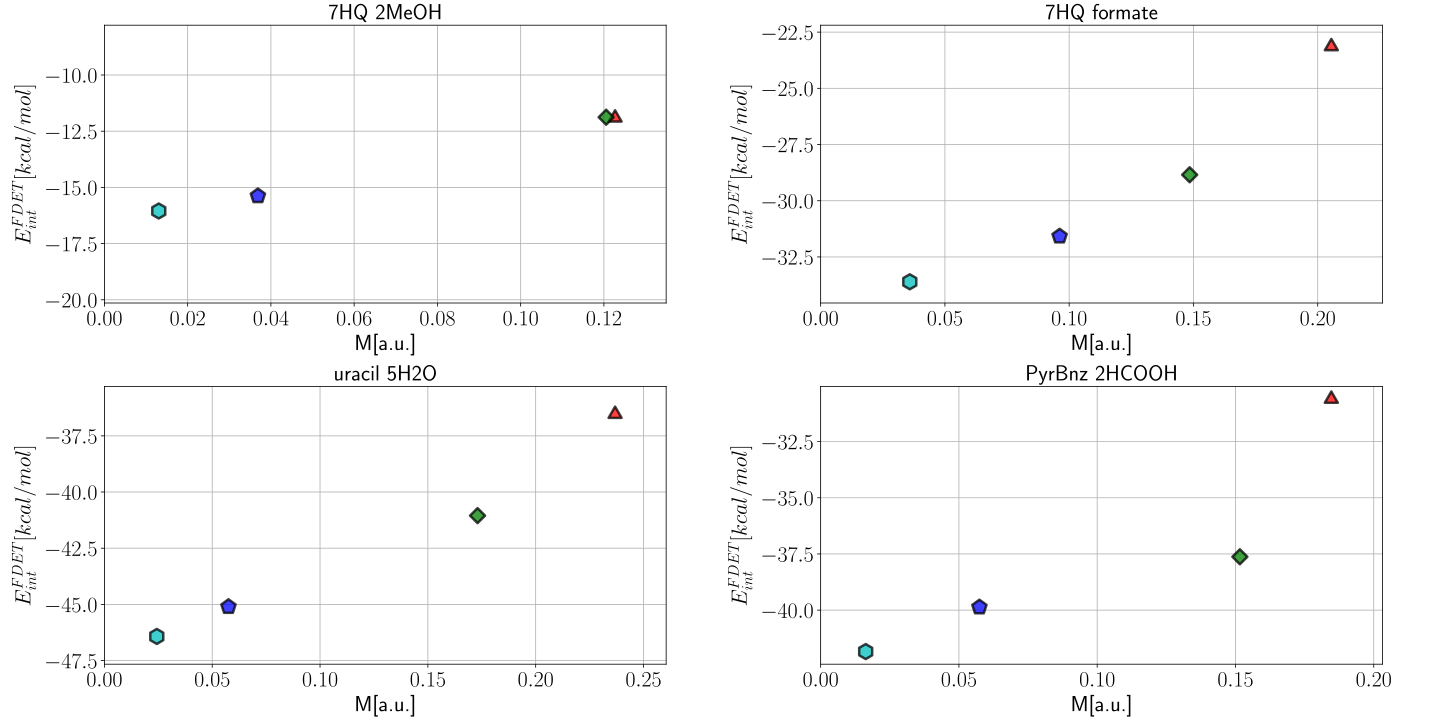
\includegraphics[width=1.0\linewidth]{M_vs_HF.png}
\caption{Integrated negative density $M$ versus $E_{HF}$, for monomer expansion calculations}
\label{fig:M_VS_HF}
\end{figure}

As one would expect, when $M[\rho^{HF}_{AB} - \rho^{HF}_{B}]$, so does $P[\rho^{o}_A, \rho_B, \rho^{HF}_{AB}]$ (cf. Fig.~\ref{fig:M_vs_P}). The value for freeze and thaw $P[\rho^{o}_A, \rho_B^{FT}, \rho^{HF}_{AB}]$ may be considered an estimate of the quality of the approximations made to obtain the embedding potential. The relation of Eq.~\ref{eq:P_bound} is respected.

\begin{figure}[H]
\centering
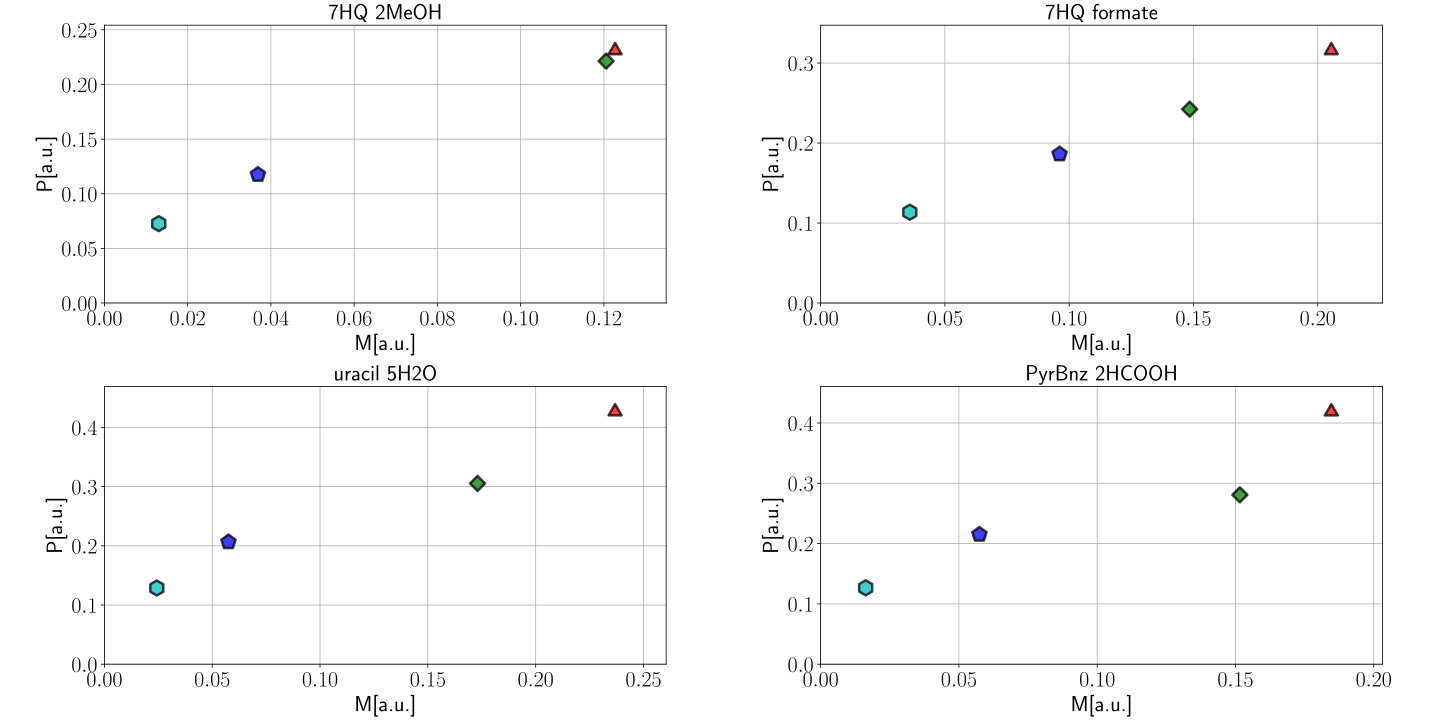
\includegraphics[width=1.0\linewidth]{M_vs_P.png}
\caption{Integrated negative density $M$ versus total density error $P$, for monomer expansion calculations}
\label{fig:M_vs_P}
\end{figure}

Within the results from FDET-MP2, shown in Fig.~\ref{fig:M_vs_MP}, lower values of $M[\rho^{HF}_{AB} - \rho^{HF}_{B}]$ lead to lower or equal energy, with only one exception.
With this level of theory, although, the improvement on the energy seems to reduce in entity at lower values of $M[\rho^{HF}_{AB} - \rho^{HF}_{B}]$, as evidenced by the smaller gap $E^{FDET-MP2}_{int}[\rho_B^{FT}] - E^{FDET-MP2}_{int}[\rho_B^{ppEC}]$, which is always smaller than **Kcal/mol, and even positive for 7Hq formate.
Albeit MP2 is not a variational mentioned, its second order energy and density corrections can be used to estimate the exact FDET energy, as outlined in subsection~\ref{sect:FDET_MP2} and in Refs.~\citenum{Wesolowski2020} and \citenum{Sen2021}. With such an approach, $E^{FDET-MP2}[\rho_B^{FT}]$ should be the lowest obtainable embedded energy with a chosen approximation of $v_{xcT}[\rho_A,\rho_B]$. In the case of 7Hq formate this is not the case. $E^{FDET-MP2}[\rho_B^{FT}]$ is, although, only ** Kcal/mol larger than the lowest value($E^{FDET-MP2}[\rho_B^{FT}]$). This can be ascribed to the fact that Eq.~\ref{eq:E_FDET_MP} is only an approximate application of Eq.~\ref{eq:E_FDET_novc}. Specifically, the second order energy correction is used instead of the full correlation energy both for $E^c_{v'}$ and $E^{HK}_{v_B}[\rho_B] = E^{HF}_{B,v_B}+E^c_{v_B}$. Furthermore, a different external potential is used in at least part of the calculation of the approximate Hohenberg-Kohn energy $\tilde{E}^{HK}_{v_B}$, and such approximation varies between $\rho_B^{FT}$ and $\rho_B^{ppEC}$, as outlined in Section~\ref{sect:comp_det}. Lastly, the incomplete basis set and higher than first order terms in the Taylor series leading to Eq.~\ref{eq:E_FDET_novc} may be playing a role.

\begin{figure}[H]
\centering
\includegraphics[width=1.0\linewidth]{M_vs_MP.png}
\caption{Integrated negative density $M$ versus $E_{MP}$, for monomer expansion calculations}
\label{fig:M_vs_MP}
\end{figure}

It is also worth mentioning that the results from $\rho_B^{FT}$ and $\rho_B^{ppEC}$ are rather good for 7Hq 2MeOH and Uracil 5H$_2$O, while they are somewhat larger for the other two systems. These results improve significantly although, when the supermolecular expansion (SE) is used. The freeze and thaw values ($E^{FDET-MP2}_{int}[\rho_B]$ and $M[\rho^{HF}_{AB} - \rho^{HF}_{B}]$) for monomer and supermolecular expansion are shown in Table~\ref{table:SE}.

\subsection{Freeze and Thaw cycles}
When a freeze and thaw procedure converges in $N$ cycles, $\frac{N}{2}$ possible densities $\rho_B^{FT,n}$ and consequently values of $M[\rho^{HF}_{AB} - \rho^{FT,n}_{B}]$ are obtained.
Two different strategies were used to obtain at each even-numbered cycle an energy to relate to the integrated negative target density: $E^{FDET-HF}_{int}[\rho_B]$, were $\rho_A$ is iteratively optimized as outlined in Section~\ref{sect:comp_det}, and linearized FDET ($E^{linFDET-HF}_{int}[\rho_B]$). 
As mentioned in Section~\ref{sect:comp_det}, linearized FDET is based on a first order Taylor expansion centered on a user-chosen density $\rho_A^{ref}$. Consequently:
\begin{equation}
 E_{xcT}^{nad}[\rho_A,\rho_B] = E_{xcT}^{nad}[\rho_A^{ref},\rho_B] + \Delta^{lin}[\rho_A,\rho_A^{ref},\rho_B],
\end{equation}
where:
\begin{equation}
 \Delta^{lin}[\rho_A,\rho_A^{ref},\rho_B]  = \int \left( \rho_A(\mathbf{r}) -  \rho_A^{ref}(\mathbf{r}) \right) \frac{\delta E_{xcT}^{nad}[\rho_A, \rho_B]}{\delta \rho_A(\mathbf{r})}
 \Bigg \vert_{\rho_A^{ref}}
 d\mathbf{r}.
\end{equation}
Since we always use $\rho_B^{FT,n-1}$ as $\rho_A^{ref}$, $\Delta^{lin}[\rho_A,\rho_A^{ref},\rho_B]$ will be zero at the end of the freeze and thaw procedure.
Fig.~\ref{fig:N_vs_HF_SE} shows $E^{FDET-HF}_{int}[\rho_B^{FT,n}]$,  $E^{linFDET-HF}_{int}[\rho_B^{FT,n}]$, and $E^{linFDET-HF}_{int}[\rho_B^{FT,n}] - \Delta^{lin}[\rho_A,\rho_A^{ref},\rho_B]$ for the first ** cycles of SE freeze and thaw.

Linearized FDET appears to be notably accurate, giving results which are almost indistinguishable from the fully self-consistent ones, for all systems, including 7Hq formate, where $\Delta^{lin}[\rho_A,\rho_A^{ref},\rho_B^{FT,0}]$ amounts to 19 Kcal/mol. 

The decrease in energy from the zero-th to the second cycle brings the energy almost to the fully converged value. Similar behavior has been observed for $M[\rho^{HF}_{AB} - \rho^{HF}_{B}]$ and $P[\rho^{o}_A, \rho_B, \rho^{HF}_{AB}]$, and is reported in the Supporting Information. Despite $E^{linFDET-HF}_{int}[\rho_B^{FT,2}]$ being almost equal to the converged value, $\Delta^{lin}[\rho_A,\rho_A^{ref},\rho_B^{FT,2}]$ may be non-negligible (e.g. 7Hq formate and PyrBnz 2HCOOH). All these observations apply to ME as well, and analogous figures are available in the Supporting Information.

\begin{figure}[H]
\centering
\includegraphics[width=1.0\linewidth]{SE_cycles_N_vs_HF.png}
\caption{$E^{FDET}[\Psi_A,\rho_B; v_B]$ with fully self-consistent calculations(blue ``X''), linearized FDET (red ``+''), and not self consistent direct calculation (red dots).}
\label{fig:N_vs_HF_SE}
\end{figure}

\section{Conclusions}
By virtue of the second Hohenberg-Kohn theorem, if $\exists \mathbf{r}$ for which $\rho^t(\mathbf{r}) < 0$, then $E^{HK}_{v_AB}[\rho_A^o + \rho_B] = E_o + \Delta E > E_o$.
No exact relation is known although between the negativity of $\rho^t$ and $\Delta E$.
We have shown how in the selected test cases decreasing values of integrated negative target density leads to a decrease in energy.
Prepolarization techniques reduce the integrated negative target density, and consequently lower the ground-state energy.

The negativity of the target density is shown to be a sizeable error contribution. As a consequence, quantifying it with a descriptor such as $M[\rho^t]$ is to be preferred when performing error analysis. Conclusions about the quality of functionals, potentials, or basis set expansions should either be drawn from calculations with the same target density or account for their difference by means of some descriptor such as $M[\rho^t]$.

Similarly, due to the energetic effect of the negativity of the target density, some type of treatment of polarization ought to be preferred when properties pertaining to a single state are concerned.
To this end, we have shown how prepolarization with point charges derived from the electrostatic potential is a well performing tradeoff.

\section{Perspective and outlook}
If excitations are considered, the error on the excitation energy is given by the difference of the energy error in each state. 
Similarly, this could be compared to the difference of integrated negative target density $M[\rho^{t, ES}] - M[\rho^{t, GS}]$, with $ES$ and $GS$ denoting the excited- and ground-state respectively.
Such differences can be expected to vary less than individual values, rendering the use of $\rho_B^{isol}$ a more reasonable choice for excitation properties than for single-state ones.
Similarly, the effect of prepolarization on $M[\rho^{t, ES}] - M[\rho^{t, GS}]$ may be expected to be harder to predict than that on each state. 

\begin{acknowledgement}
The authors thank funding xyz.
\end{acknowledgement}

\begin{suppinfo}
The data is provided in csv.
\begin{itemize}
  \item Filename: data as comma separated values. The labels are explaind below:
  \begin{itemize}
   \item label: explanation
  \end{itemize}


\end{itemize}

\end{suppinfo}

%%%%%%%%%%%%%%%%%%%%%%%%%%%%%%%%%%%%%%%%%%%%%%%%%%%%%%%%%%%%%%%%%%%%%
%% The appropriate \bibliography command should be placed here.
%% Notice that the class file automatically sets \bibliographystyle
%% and also names the section correctly.
%%%%%%%%%%%%%%%%%%%%%%%%%%%%%%%%%%%%%%%%%%%%%%%%%%%%%%%%%%%%%%%%%%%%%
\bibliography{group_bibliography}

\end{document}
